% ---
\documentclass{article}


% Packages
% ---
\usepackage{amsmath,amssymb,amsthm} 	% Advanced math typesetting
% \usepackage[utf8]{inputenc} 	% Unicode support (Umlauts etc.)
\usepackage[USenglish]{babel} 	% Change hyphenation rules
\usepackage{hyperref} 				% Add a link to your document
\usepackage{graphicx}				% Add pictures to your document
\graphicspath{ {./images/} }	% image directory
\usepackage{listings} 				% Source code formatting and highlighting
\lstset{basicstyle=\ttfamily}		%Typewriter font for code writing
\usepackage{geometry}
\geometry{margin=1in}
\usepackage{enumitem}
\usepackage{float}
%\floatstyle{boxed}
\restylefloat{figure}
\usepackage{mathabx}
\usepackage{fancyhdr}
\usepackage[dvipsnames]{xcolor}
\usepackage{scrextend}

% Colors
\definecolor{blu}{rgb}{0,0,1}
\def\blu#1{{\color{blu}#1}}
\definecolor{gre}{rgb}{0,.5,0}
\def\gre#1{{\color{gre}#1}}
\definecolor{red}{rgb}{1,0,0}
\def\red#1{{\color{red}#1}}
\def\norm#1{\|#1\|}

\theoremstyle{definition}
\newtheorem{definition}{Def}
\newcommand{\centerfig}[2]{\begin{center}\includegraphics[width=#1\textwidth]{#2}\end{center}}

\pagestyle{fancy}
\fancyhf{}
\lhead{\bf CPSC 340 \\ Week 3 }
\rhead{\bf Jeremi Do Dinh \\ 61985628}
\rfoot{Page \thepage}



\usepackage{tikz}						% Graph drawing tools
\usetikzlibrary {positioning}

\usepackage{breqn}
\usepackage{multicol} 				% Multiple column functionality
\usepackage{blindtext}


\begin{document}

\noindent \url{https://www.cs.ubc.ca/~fwood/CS340/}

\section*{Lecture VI}
\textbf{January 20th, 2020}\\
\noindent \url{https://www.cs.ubc.ca/~fwood/CS340/lectures/L6.pdf}

\subsection*{Laplace Smoothing}
Currently we have the following estimate:
\begin{align*}
	P(\text{'lactase'} = 1 | \text{"spam}) = \frac{\text{\# spam messages with lactose}}{\text{\# of spam messages}}
\end{align*}
But there is a problem if there are {\color{OliveGreen} no spam messages with "lactase"}. This then means that $ P(\text{'lactase'} = 1 | \text{"spam}) = 0 $, so {\color{red} all spam messages with "lactase" get through automatically. } \\ \\
To fix this we use \textbf{\color{blue} Laplace smoothing}:
\begin{itemize}
	\item Add 1 to the numerator
	\item add 2 to the denominator
\end{itemize}
This acts as a 'fake' spam example that has lactase, and a 'fake' spam example that doesn't:{ \color{blue}
\begin{align*}
\frac{\text{\# spam messages with lactose}+1}{\text{\# of spam messages}+2}
\end{align*}}
Typically, we {\color{OliveGreen} do this for all features}. It helps against overfitting, by biasing towards the uniform distribution. \\
A common variation is to use a {\color{OliveGreen} real number $ \beta $} rather than 1. We {\color{OliveGreen} add $ \beta k $ to the denominator}, if the feature has $ k $ possible values (so it sums to 1). 
\begin{align*}
	P(x_{ij} = c | y_i = class) \approx \frac{\text{(\# of examples with $ x_{ij} = c $)} + \beta}{\text{\# of examples in class} + \beta k}
\end{align*}
This is a {\color{blue} "maximum a posteriori}" (MAP) estimate of the probability

\subsection*{Decision Theory}
We ask the question of whether we are equally concerned about "spam" and "not spam". For this we consider the cost associated with the different scenarios, namely True positives, true negatives, false positives and false negatives. Costs may vary, since:
\begin{itemize}
	\item Letting a spam message through (false negative) is not a big deal.
	\item Filtering a not spam (false positive) message will make users mad.
\end{itemize}
Consider the following costs:
\begin{figure}[H]
	\centering
	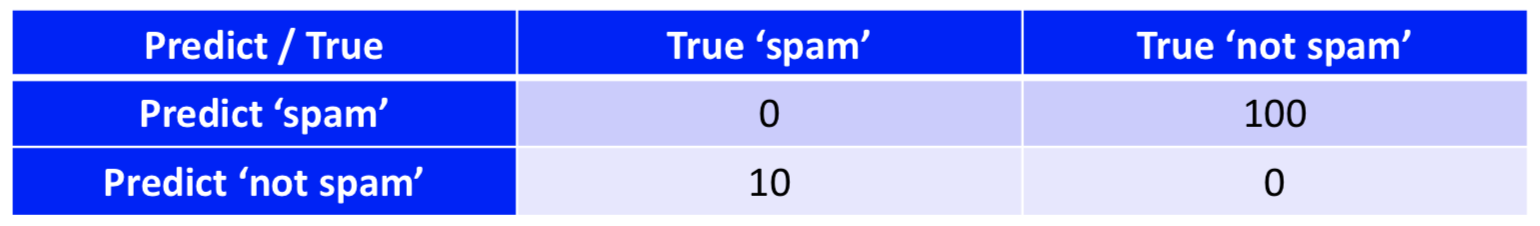
\includegraphics[width = 4in]{Pic1}
\end{figure}
In this case, instead of taking the most probable model, we use the model $ \hat{y_i} $ that {\color{OliveGreen} minimizes the expected cost}:
\begin{align*}
\mathbb{E}[\text{cost}(\hat{y_i}, \tilde{y_i})]
\end{align*}
Even if "spam" has a higher probability, predicting "spam" has expected higher cost.
\textbf{Example:}\\
Consider a test example where we have $ P(\tilde{y_i}=\text{"spam"} | \tilde{x_i}) = 0.6 $. Then:
\begin{align*}
	\mathbb{E}[\text{cost}(\hat{y_i} = \text{"spam"}, \tilde{y_i})] &= P(\tilde{y_i}=\text{"spam"} | \tilde{x_i})\text{cost}(\hat{y_i} = \text{"spam"}, \tilde{y_i}\text{"spam"}) + \\ & \quad P(\tilde{y_i}=\text{"not spam"} | \tilde{x_i})\text{cost}(\hat{y_i} = \text{"spam"}, \tilde{y_i} = \text{"not spam"}) \\
	&= (0.6)(0) + (0.4)(100) \\
	&= 40 \\
	\mathbb{E}[\text{cost}(\hat{y_i} = \text{"not spam"}, \tilde{y_i})] &= (0.6)(10) + (0.4)(0) \\ &= 6
\end{align*}
Even though "spam" is more likely, we should predict "not spam".
\subsection*{Decision Trees vs. Naïve Bayes}
\begin{multicols}{2}
	\textbf{Decision Trees}
	\begin{enumerate}
		\item Sequence of rules based on 1 feature.
		\item Training: 1 pass over data per depth.
		\item Greedy splitting as approximation.
		\item Testing: just look at features in rules.
		\item New data: might need to change tree.
		\item Accuracy: good if simple rules based on individual features work (“symptoms”).
	\end{enumerate}
\textbf{Naïve Bayes}
\begin{enumerate}
	\item Simultaneously combine all features.
	\item Training: 1 pass over data to count.
	\item Conditional independence assumption.
	\item Testing: look at all features.
	\item New data: just update counts.
	\item Accuracy: good if features almost independent given label (bag of words).
\end{enumerate}

\end{multicols}
\subsection*{K-Nearest Neighbors (KNN)}
This is an old and simple classifier. To classify an example $ \tilde{x_i} $, we:
\begin{enumerate}
	\item Find the {\color{OliveGreen} 'k' training examples that are "nearest"} to $ x_i $
	\item Classify using the {\color{OliveGreen} most common label} of “nearest” training examples.
\end{enumerate}
\begin{figure}[H]
	\centering
	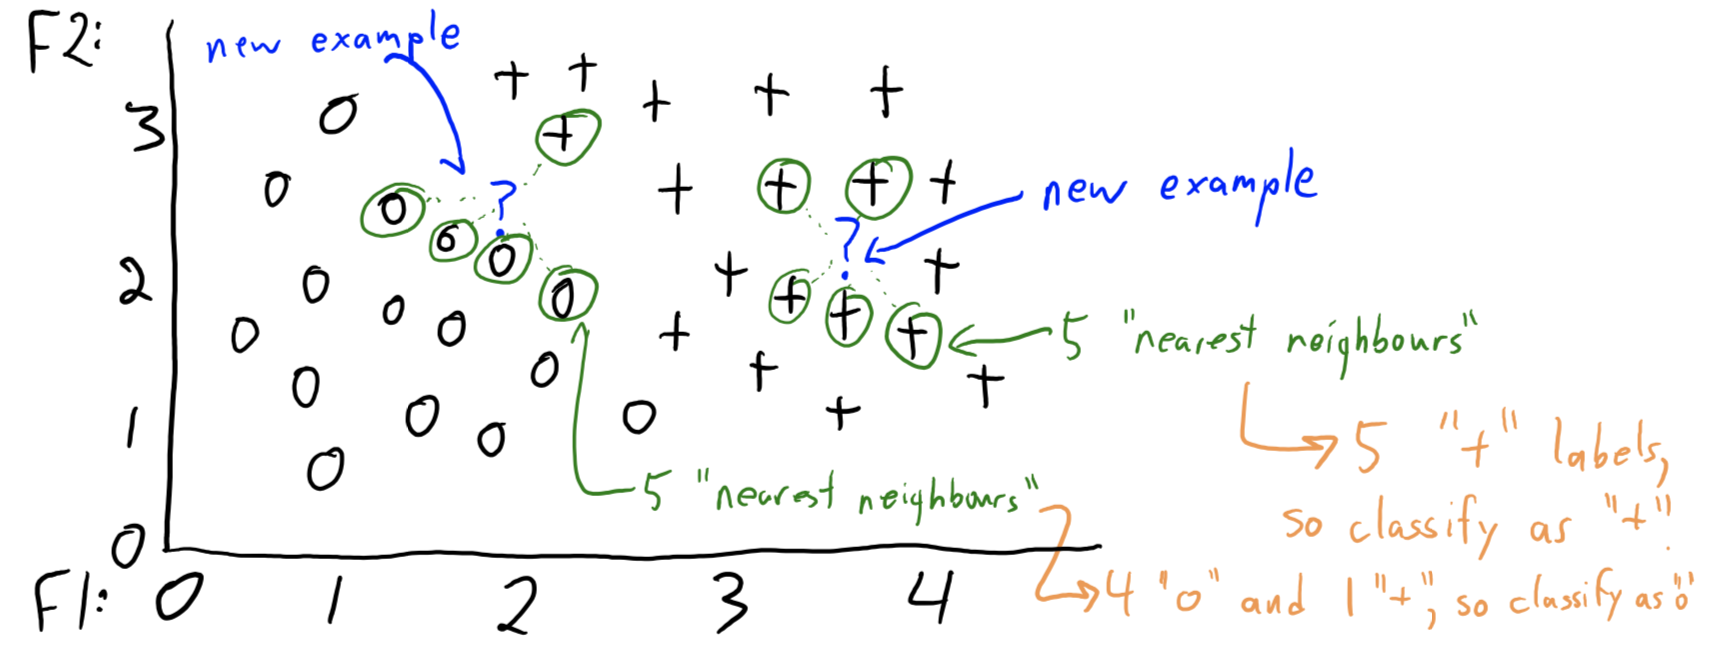
\includegraphics[width = 5in]{Pic2}
	\caption{KNN example}
\end{figure}
\textbf{Assumption}: {\color{OliveGreen} Examples with similar features, are likely to have similar labels}. This seems strong, but basically {\color{OliveGreen} all good classifiers rely on this assumption}:
\begin{enumerate}[label=-]
	\item If not true there may be nothing to learn and you are in “no free lunch” territory.
	\item Methods just differ in how you define “similarity”.
\end{enumerate}
The most common distance function is the {\color{blue} Euclidean distance}:
\begin{align*}
||x_i - \tilde{x_{i'}} || = \sqrt{\sum_{j = 1}^{d}(x_{ij} - \tilde{x_{i'j}})^2}
\end{align*}
Here, $ x_i $ is the feature vector of the training example $ i $, and $ \tilde{x_{i'}} $ is the feature vector of test example $ i' $. It costs $ O(d) $ to calculate this for pairs of examples.
\subsubsection*{Effect of $ k $ (hyperparameter) in KNN}
If $ k $ is large, then the model will be very simple, for instance if $ k=n $, the we just compute the mode of the labels. The model {\color{OliveGreen} gets more complicated as $ k $ decreases}.
\begin{figure}[H]
	\centering
	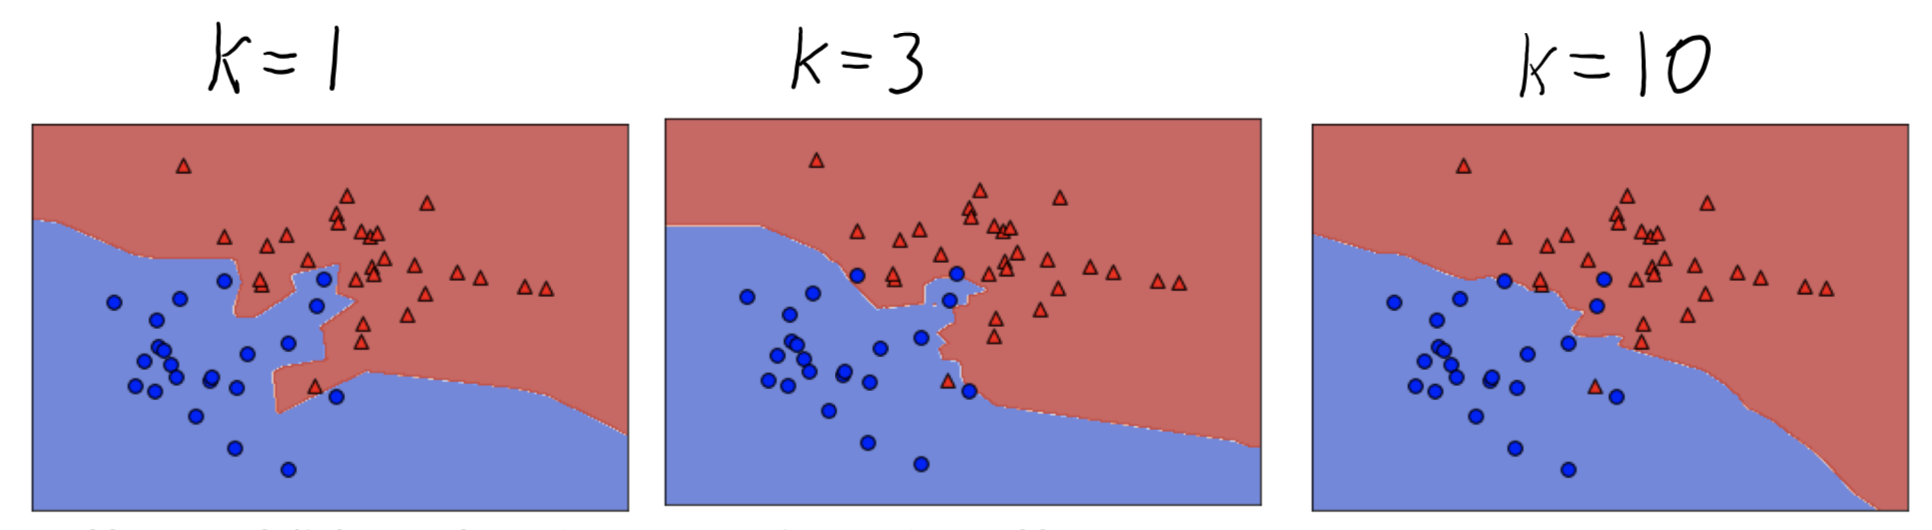
\includegraphics[width = 6in]{Pic3}
	\caption{Effect of the value of $ k $ on the model}
\end{figure}
\noindent Fundamental trade-off: {\color{OliveGreen} As $ k $ increases, training error increases, but approximation error decreases. }

\begin{figure}[H]
	\centering
	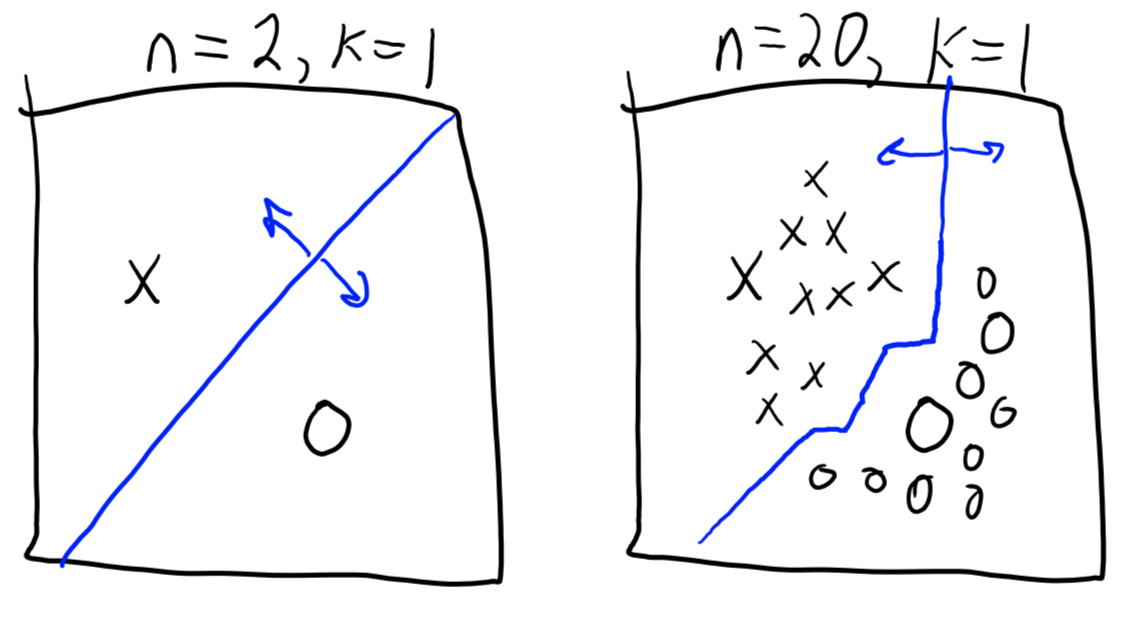
\includegraphics[width = 3in]{Pic5}
	\caption{When $ k $ is small, the model can be very simple, but gets more complicated as $ n $ increases}
\end{figure}

\subsubsection*{KNN Implementation}
There is {\color{OliveGreen} no training} phase in KNN (lazy learning)
\begin{itemize}
	\item You just store the training data
	\item Costs $ O(1) $ if you just use a pointer
\end{itemize}
But {\color{red} Predictions are expensive}: $ O(nd) $ to classify one example
\begin{itemize}
	\item Need to do O(d) distance calculation for all ‘n’ training examples.
	\item So {\color{OliveGreen} prediction time grows with number of training examples.}
\end{itemize}
But {\color{red} Storage is expensive}: needs $ O(nd) $ of memory to store $ X $ and $ y $. 
\begin{itemize}
	\item So {\color{OliveGreen} memory grows with number of training examples.}
	\item When storage depends on ‘n’, we call it a \textit{\color{blue} non-parametric} model
\end{itemize}
\subsection*{Parametric vs. Non-parametric models}
\textbf{Parametric Models}
\begin{itemize}
	\item Have a fixed number of parameters: {\color{OliveGreen} trained “model” size is $ O(1) $ in terms $ n $.}
	\item You can estimate the fixed parameters more accurately with more data.
	\item But {\color{OliveGreen} eventually more data doesn’t help}: model is too simple
\end{itemize}
\textbf{Non-parametric models}
\begin{itemize}
	\item {\color{OliveGreen} Number of parameters grows with ‘n’}: size of “model” depends on ‘n’.
	\item Model gets {\color{OliveGreen} more complicated as you get more data.}
\end{itemize}
\textbf{\color{OliveGreen} Parametric models have bounded memory}\\
\textbf{\color{red} Non-parametric models have unbounded memory}
\begin{figure}[H]
	\centering
	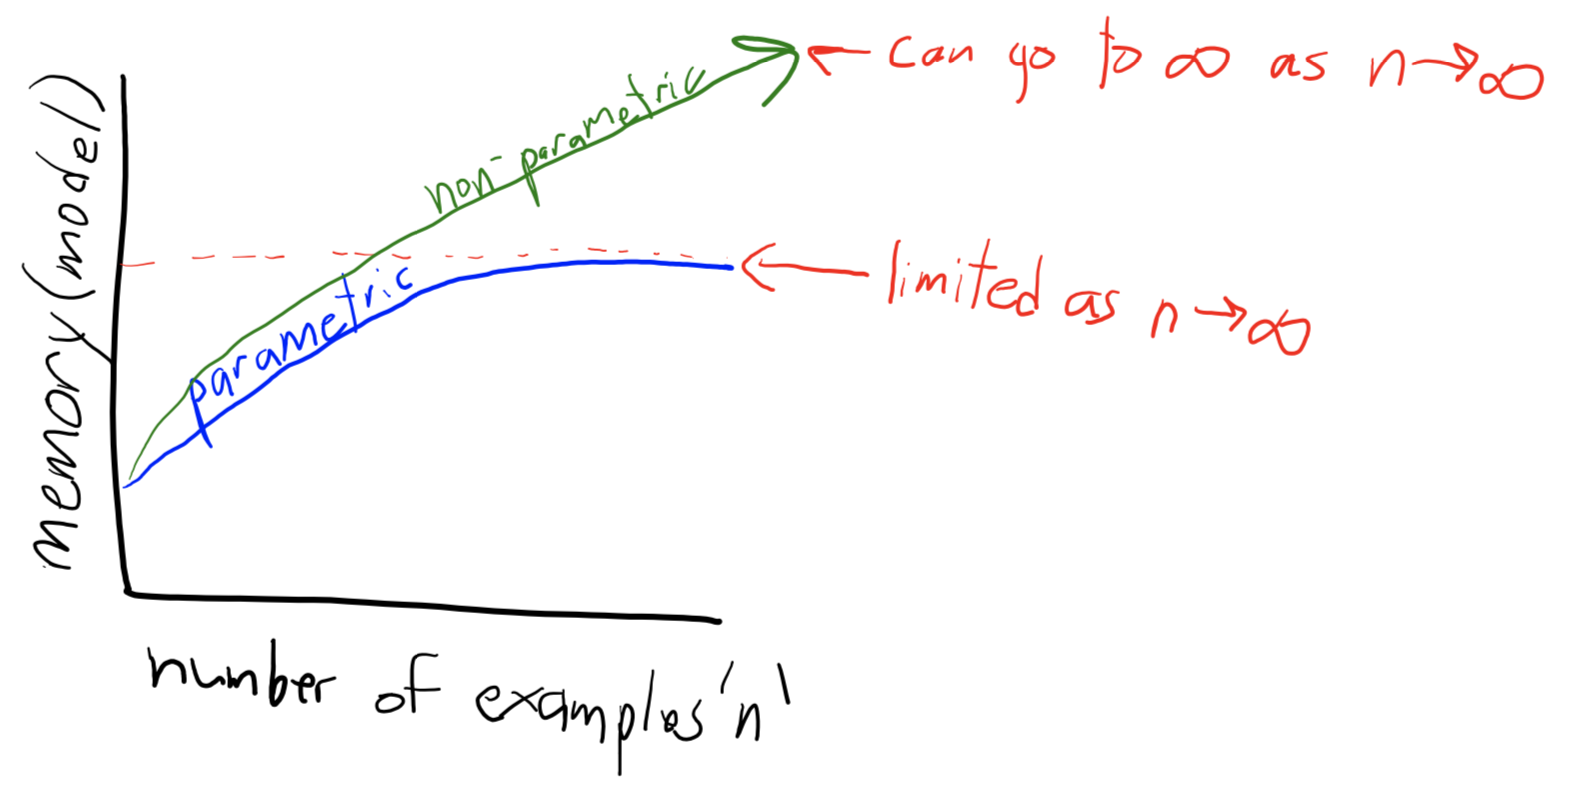
\includegraphics[width = 4in]{Pic4}
	\caption{Comparison of memory usage of Parametric vs. Non-parametric models}
\end{figure}

\section*{The curse of Dimensionality}
The \textbf{\color{blue} curse of dimensionality} is used to describe the problems associated with high-dimensional spaces. 
\begin{itemize}
	\item Volume of space grows {\color{red} exponentially} with dimension.
	\item Need {\color{red} exponentially more points} to ‘fill’ a high-dimensional volume.
	\begin{itemize}
		\item Nearest” neighbors might be really far even with large $ n $.
	\end{itemize}
\end{itemize}

\newpage
\section*{Lecture VII}
\textbf{January 22nd, 2020}\\
\url{https://www.cs.ubc.ca/~fwood/CS340/lectures/L7.pdf}
\subsection*{Norms}
\subsection*{Decision Trees vs. Naïve Bayes vs. KNN}
\subsection*{Application: Optical Character Recognition}
\subsection*{Application: Body-Part Recognition}
\subsection*{Ensemble Methods}
Ensemble methods are \blu{classifiers, that take classifiers as input}. They often have higher accuracy than input classifiers. \\
Remember the fundamental trade off:
\begin{enumerate}
	\item $ E_{\text{train}} $: How small can you make the training error \blu{vs.}
	\item $ E_{\text{approx}} $: How well the training error approximate the testing error.
\end{enumerate}
We have that the goal of ensemble methods is that meta classifier:
\begin{itemize}
	\item Does much better on does much better on one of these, than individual classifiers
	\item Doesn’t do too much worse on the other.
\end{itemize}
This suggests two types of ensemble methods:
\begin{enumerate}
	\item \blu{Boosting:} improves training error of classifiers with high $ E_{\text{train}} $
	\item \blu{Averaging:} improves approximation error of classifiers with high $ E_{\text{approx}} $
\end{enumerate}

\subsubsection*{Averaging}
The input to \blu{averaging} is the prediction of a set of models:
\begin{itemize}
	\item Decision trees make one prediction. 
	\item Naive Bayes makes another prediction
	\item KNN makes another
\end{itemize}
The simple model averaging then takes the \gre{mode of the predictions} or average probabilities if it is probabilistic. 
\centerfig{0.85}{Pic11}

\begingroup
\leftskip1em
\subsubsection*{Digression: Stacking}
A common variation of this method is called \textbf{stacking}. We \gre{fit another classifier} that uses the predictions as features.
\centerfig{0.90}{Pic12}
\endgroup

\subsubsection*{Why can Averaging work?}
Consider 3 binary classifiers, \gre{each independently correct} with probability 0.80. With simple averaging, ensemble is correct if we have “at least 2 right”:
\begin{itemize}
	\item  $ P(\text{all 3 right}) = 0.83 = 0.512 $.
	\item $ P(\text{2rights,1wrong})=3\times0.82(1-0.8)=0.384. $
	\item$  P(\text{1 right,2 wrongs})=3 \times (1-0.8)20.8=0.096. $
	\item $ P(\text{all 3 wrong}) = (1-0.8)\times 3 = 0.008. $
	\item So ensemble is right with probability 0.896 (which is $ 0.512+0.384 $).
\end{itemize}
\textbf{Notes:}
\begin{itemize}
	\item For averaging to work, \gre{classifiers need to be at least somewhat independent}
	\item You also want the probability of being right to be $ > 0.5 $ otherwise it will do much worse. 
	\item We also don't want the probabilities to be too different, otherwise it might be better to use the most accurate one
\end{itemize}
\textbf{Intuition}
If we consider classifiers that over-fit (like deep decision trees), if they all overfit in exactly the same way, then the averaging does nothing. \\ \\
However if they all make \blu{independent errors}, then the probability that the average is wrong can be lower than for each classifier, since we pay less attention to specific over-fitting of each classifier.

\subsection*{Random Forests}
Random Forests \blu{average a set of deep decision trees}. It tends to be \gre{one of the best "out of the box" classifiers}. It's often close to the best performance of any method on the first run, and \gre{predictions are very fast}. \\ \\
We have that deep decision trees don't make independent errors, since for each training set the decision tree is the same. therefore we have two key ingredients in Random Forests:
\begin{enumerate}
	\item \blu{Bootstrapping}
	\item \blu{Random trees}
\end{enumerate}
\subsubsection*{Bootstrap sampling}
\begingroup
\leftskip2em
\textbf{Example}
We start with a deck of 52 cards, and sample 52 cards with replacement, such that the cards from each of the 52 samples form a new deck of 52 cards (of which some may be duplicates).\\
The new 52 deck card is called the \textbf{\blu{"bootstrap sample"}}:
\begin{itemize}
	\item Some \gre{cards will be missing}, and some \gre{cards will be duplicated}, so calculations on the bootstrap sample will give different results than original data.
	\item However, the bootstrap sample roughly maintains trends:
	\begin{itemize}
		\item Roughly 25\%of the cards will be diamonds.
		\item Roughly 3/13 of the cards will be “face” cards.
		\item There will be roughly four “10” cards.
	\end{itemize}
\item A common use is to compute a statistic based on \gre{several bootstrap samples}. This gives you an idea of \gre{how the statistic varies as you vary the data}.
\end{itemize}
\endgroup
\subsubsection*{Random Forest Ingredient 1: Bootstrap}
\textbf{\blu{Bootstrap sample}} of a list of ‘n’ examples: a new \blu{set of size ‘n’ chosen independently with replacement}:
\begin{lstlisting}[tabsize=2]
		for i in 1:n:
			j = rand(1:n)							# pick a random number from {1, ..., n}
			X_bootstrap[i,:] = X[j,:]		# use the random sample
\end{lstlisting}
Gives new data set of $ n $ examples, with some duplicated and some missing. For large $ n $, approximately 63\% of original examples are included. \\ \\
\textbf{\blu{Bagging}}: using bootstrap samples for ensemble learning:
\begin{itemize}
	\item Generate several \gre{bootstrap samples of the examples $ (x_i,y_i) $}
	\item Fit a \gre{classifier to each bootstrap} sample.
	\item At test time, \gre{average the predictions}.
\end{itemize}
Therefore \textbf{\blu{Random Forests}} are an ensemble method that averages the results of fitting deep \blu{random trees} to \blu{bootstrap samples} of data. The randomization \textbf{\gre{encourages errors of different trees to be independent}}.
\centerfig{0.80}{Pic13}
\centerfig{0.80}{Pic14}

\subsubsection*{Random Forest Ingredient 2: Random Trees}
For \gre{each split} in \blu{a random tree}:
\begin{itemize}
	\item \gre{randomly sample} a small number of possible features (typically $ \sqrt{d} $). 
	\item \red{Only consider these random features} when searching for the optimal rule
\end{itemize}
\centerfig{0.80}{Pic15}
\centerfig{0.80}{Pic16}

\begin{itemize}
	\item Splits will tend to use different features in different trees. they will still overfit, but hopefully errors will be more independent.
	\item So the average tends to \gre{have a much lower test error}.
	\item Empirically,random forests are one of the “best” classifiers.
\end{itemize}

\newpage

\section*{Lecture VIII}
\textbf{January 24th, 2020}\\
\url{https://www.cs.ubc.ca/~fwood/CS340/lectures/L8.pdf}
\subsection*{Unsupervised learning}
In \textbf{Supervised learning}, we have:
\begin{itemize}
	\item Features $ x_i $ and class labels $ y_i $
	\item We write a program that produces $ y_i $ from $ x_i $.
\end{itemize}
In \textbf{Unsupervised learning}:
\begin{itemize}
	\item We \red{\textbf{only have $ x_i $ values}}, but no specific target labels
	\item We want to do something with them 
\end{itemize}
Some \textit{supervised learning tasks are}:
\begin{itemize}
	\item Outlier detection: Is it a 'normal' $ x_i $?
	\item Similarity search: which examples look like this $ x_i $?
	\item Association rule: Which $ x^j $ occur together?
	\item Latent-factors: What ‘parts’ are the $ x_i $ made from?
	\item Data visualization: What does the high-dimensional $ X $ look like?
	\item Ranking: Which are the most important $ x_i $?
	\item \blu{Clustering: What types of $ x_i $ are there?}
\end{itemize}



\subsection*{Clustering}
\textbf{Input:} set of examples described by features $ x_i $ \\ \\
\textbf{Output:} an \blu{assignment of examples to ‘groups’} \\ \\
\textbf{Note:} Unlike classification, \red{we are not given the groups}. This means that the Algorithm must \blu{discover the groups}

\begingroup
\leftskip1em
	\subsubsection*{Example}
	\begin{figure}[H]
	\centering
	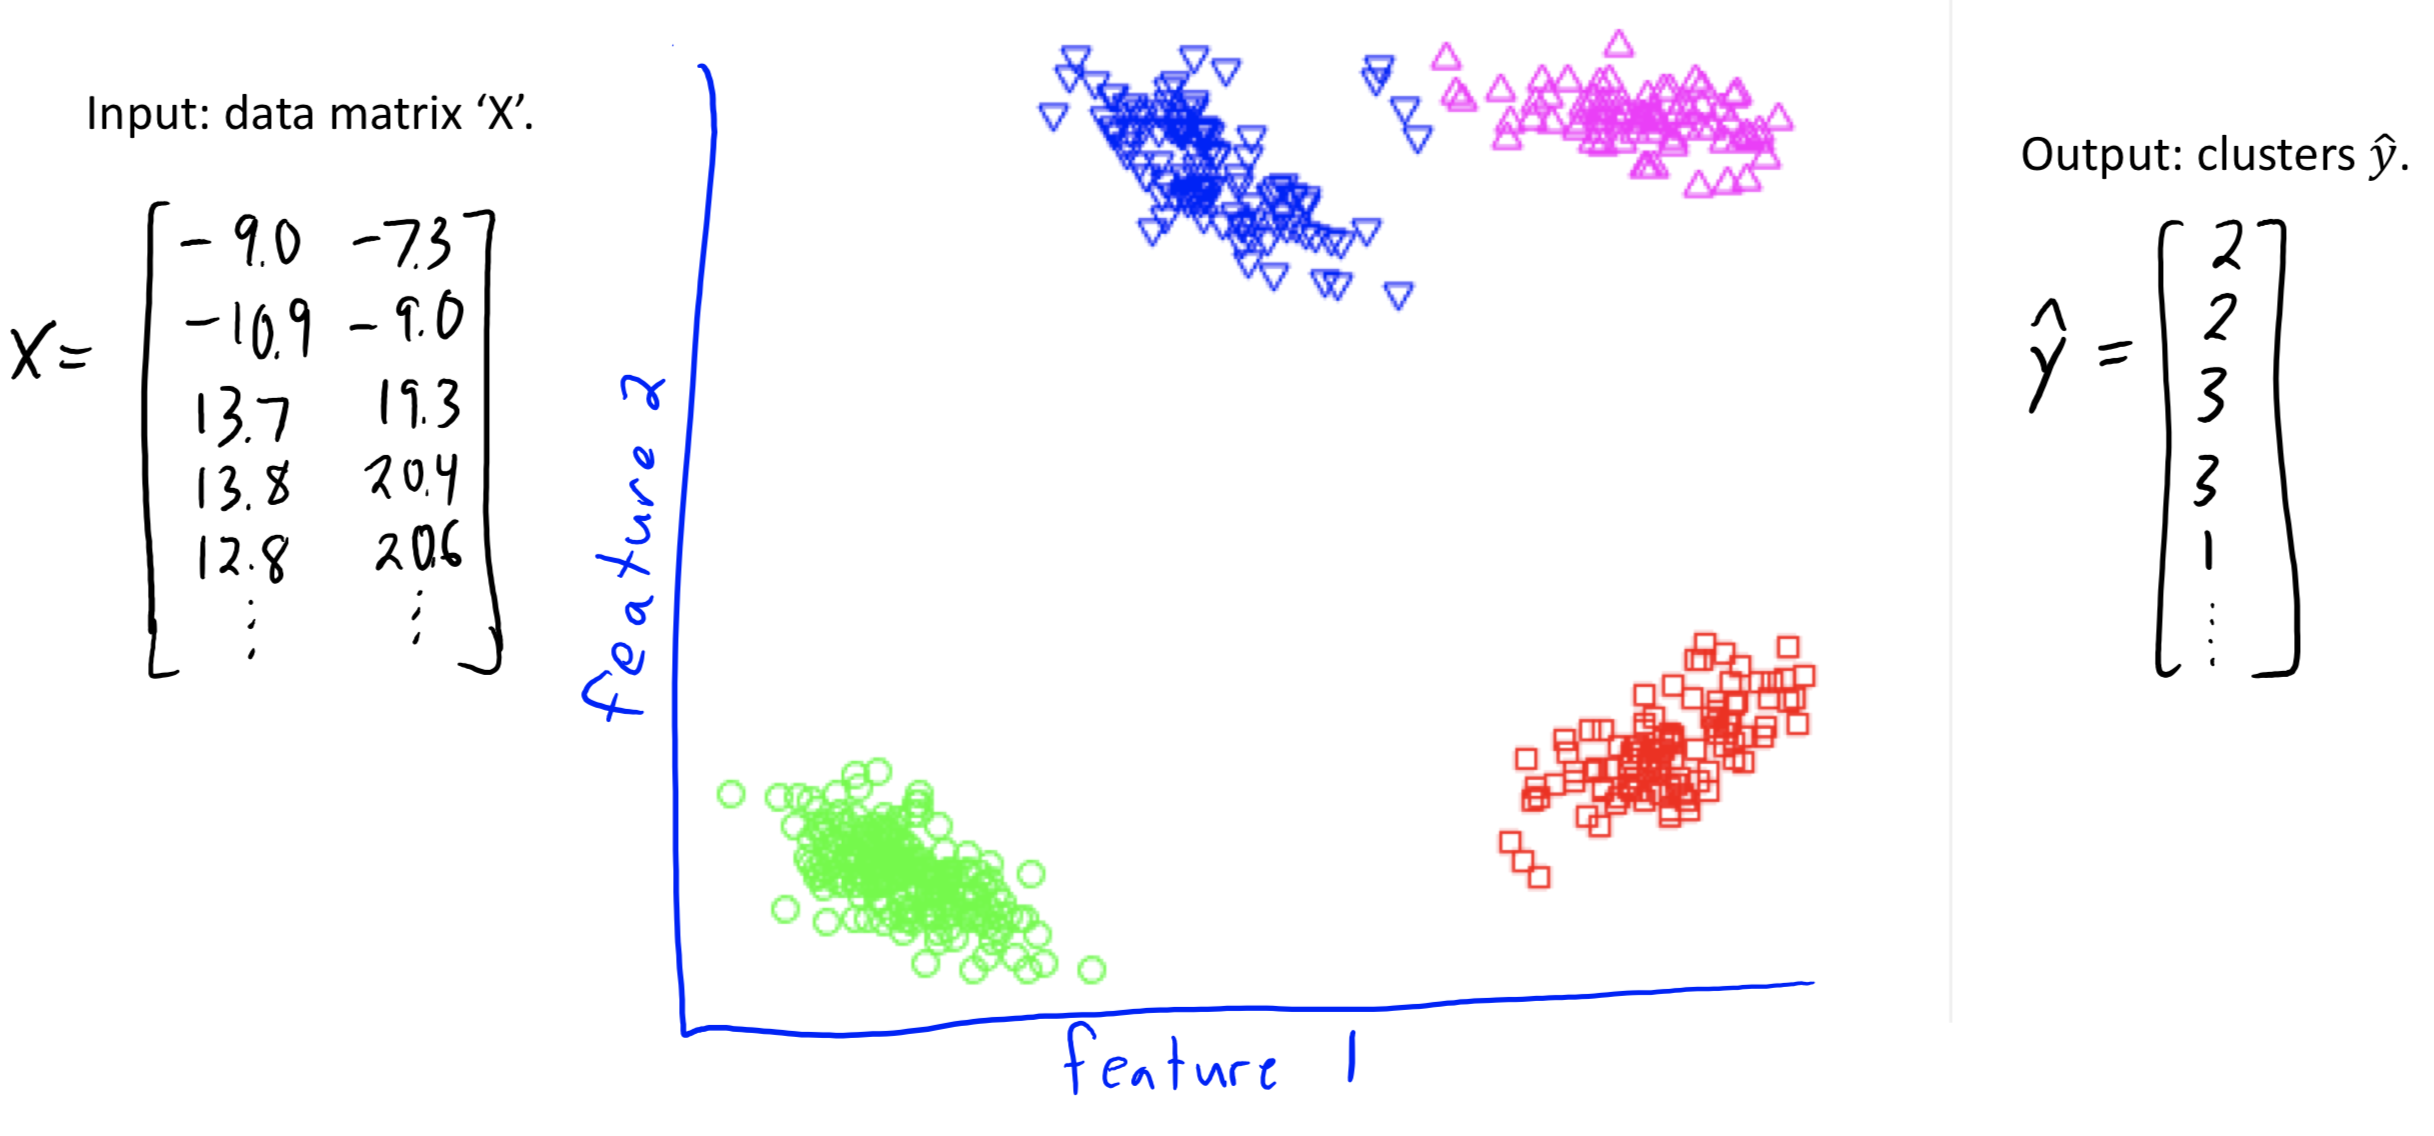
\includegraphics[width = 4.5in]{Pic6}
	\caption{Example of clustering}
	\end{figure}

\endgroup

\subsubsection*{Data clustering}
The general goal of clustering algorithms is that \blu{examples in the \textbf{same group should be 'similar'}}, and \blu{examples in \textbf{different groups should be 'different'.}}\\ \\
But the 'best' clustering is hard to define, since \red{we don't have a test error}. This means that generally there is no best method in unsupervised learning: so there are lots of methods and we’ll focus on important/representative ones. \\\\
So why cluster?
\begin{itemize}[label = -]
	\item We could want to \gre{know what the different groups are.}
	\item We could want to \gre{find the group for a new example $ x_i $.}
	\item We could want to \gre{find examples related to a new example $ x_i $.}
	\item We could want a \gre{‘prototype’ example for each group.}
\end{itemize}






\subsection*{K-means}

The most popular clustering technique is called K-means. As \textbf{Input} we have:
\begin{itemize}
	\item The \blu{number of clusters 'k' (hyper-parameter)}
	\item \blu{Initial guess of the center (the mean) of each cluster}
\end{itemize}
The \textbf{Algorith works as follows}:
\begin{itemize}
	\item \blu{Assign $ x_i $} to its closest mean
	\item \blu{Update the means} based on the assignment 
	\item Repeat until convergence
\end{itemize}
\begingroup
\leftskip1em
\subsubsection*{Example}

\begin{figure}[H]
	\centering
	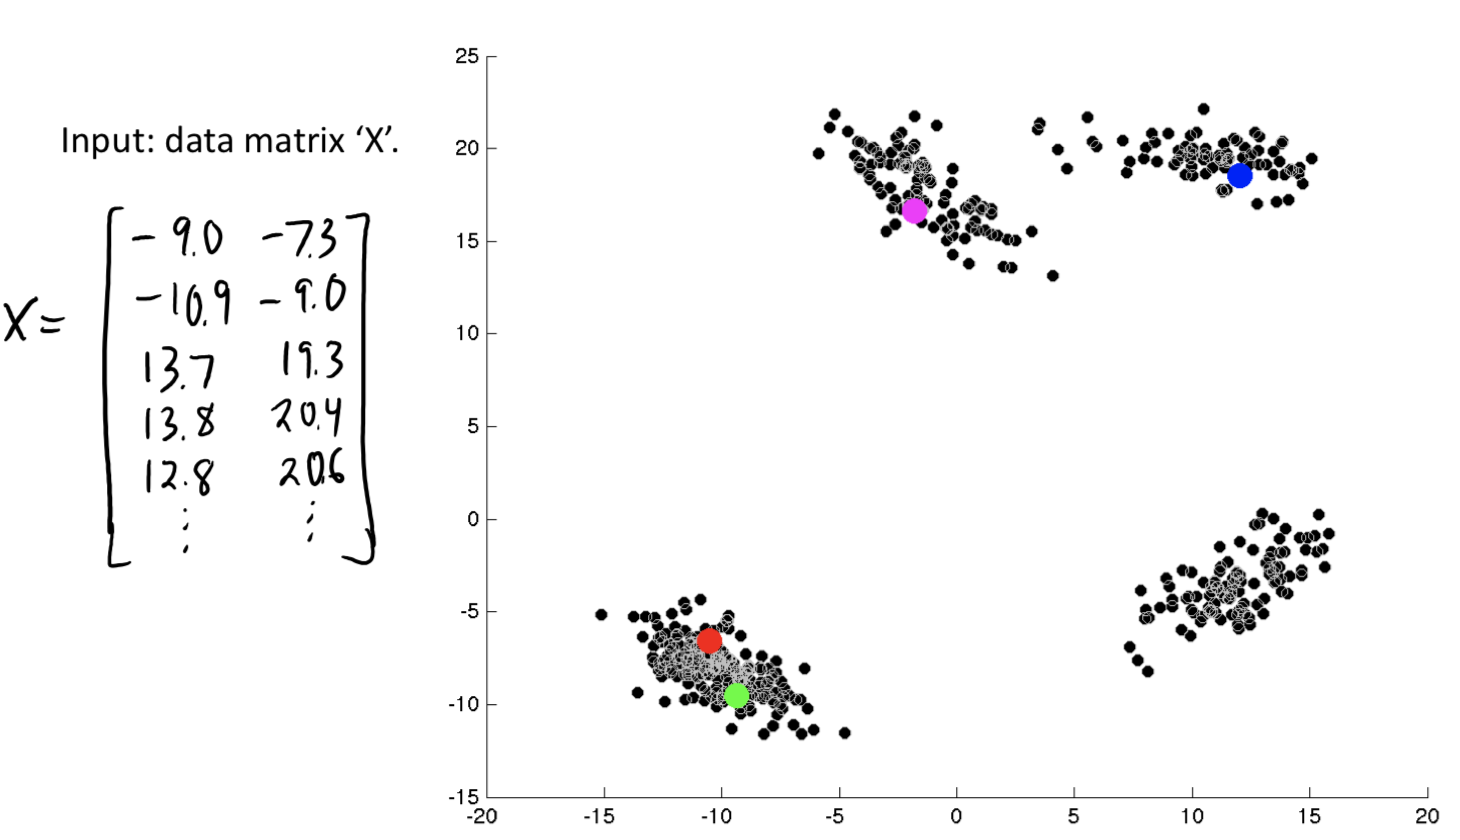
\includegraphics[width = 4.5in]{Pic7}
	\caption{Start with $ k $ initial ‘means’ (usually, random data points)}
\end{figure}
\begin{figure}[H]
	\centering
	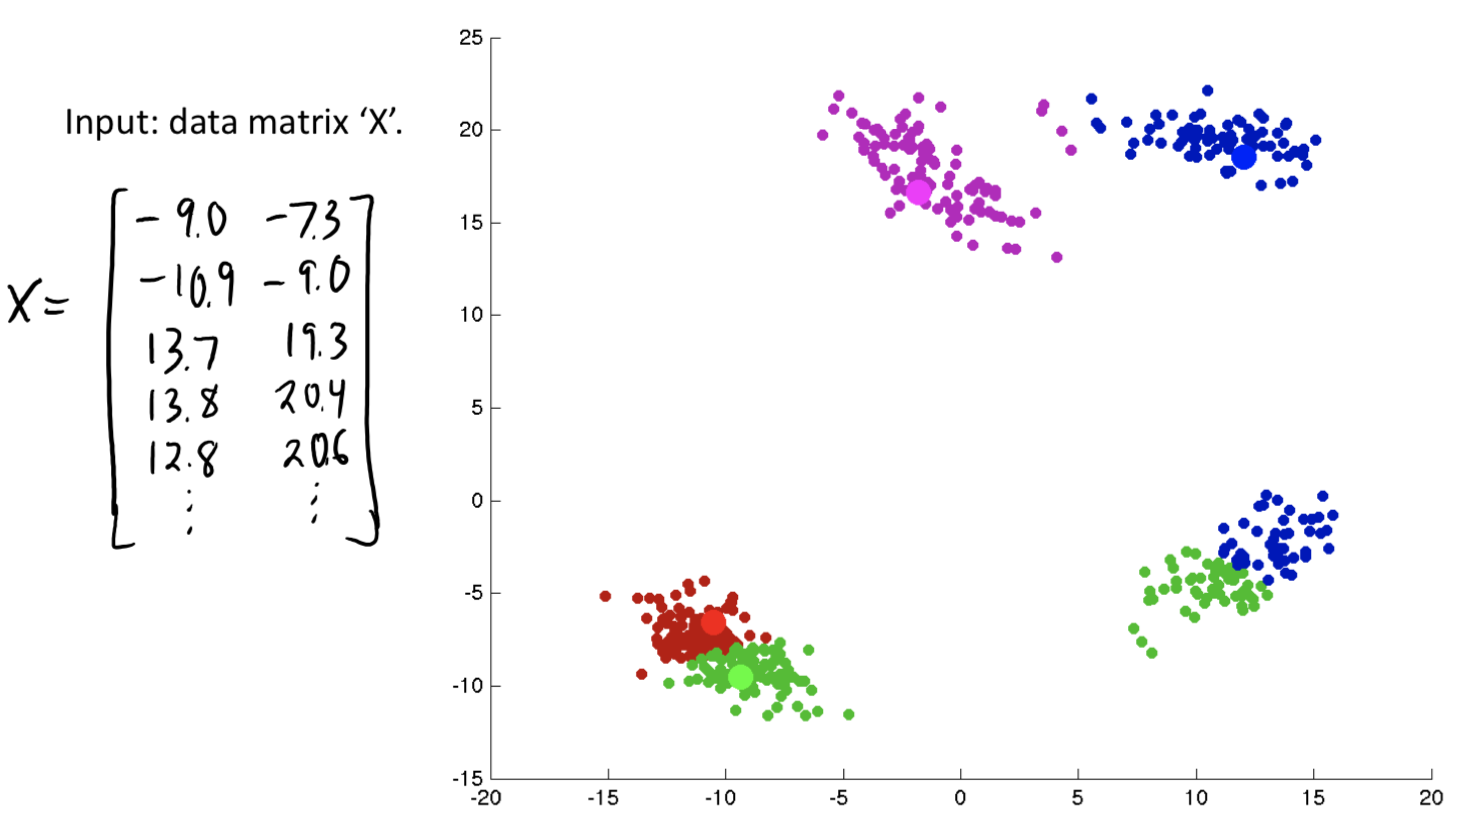
\includegraphics[width = 4.5in]{Pic8}
	\caption{Assign each example to the closest mean.}
\end{figure}
We then update the mean of each group, until no data points change groups 
\endgroup
\subsubsection*{K-Means Issues}
K-means is \gre{guaranteed to converge when we use euclidean distance}. Given a new test example, we \gre{assign it to the nearest mean to cluster it}. However:
\begin{itemize}
	\item K-means assumes that \red{you know the number of clusters $ k $}: there are lots of heuristics to pick $ k $, but none are satisfying. 
	\item Each example is assigned to \red{one, and only one cluster}. There is no possibility of overlapping clusters or leaving examples unassigned. 
	\item It may converge to a \red{sub-optimal solution}. 
\end{itemize}
Since k-means may depend on how the problem was initialized, then it is good practice to start the problem with different initializations, and find the best fit. This is called \blu{random restarts}, where we choose several random initialization points, and choose the best one. 

\subsubsection*{KNN vs. K-means}
They are \gre{not to be confused!!!}
\begin{figure}[H]
	\centering
	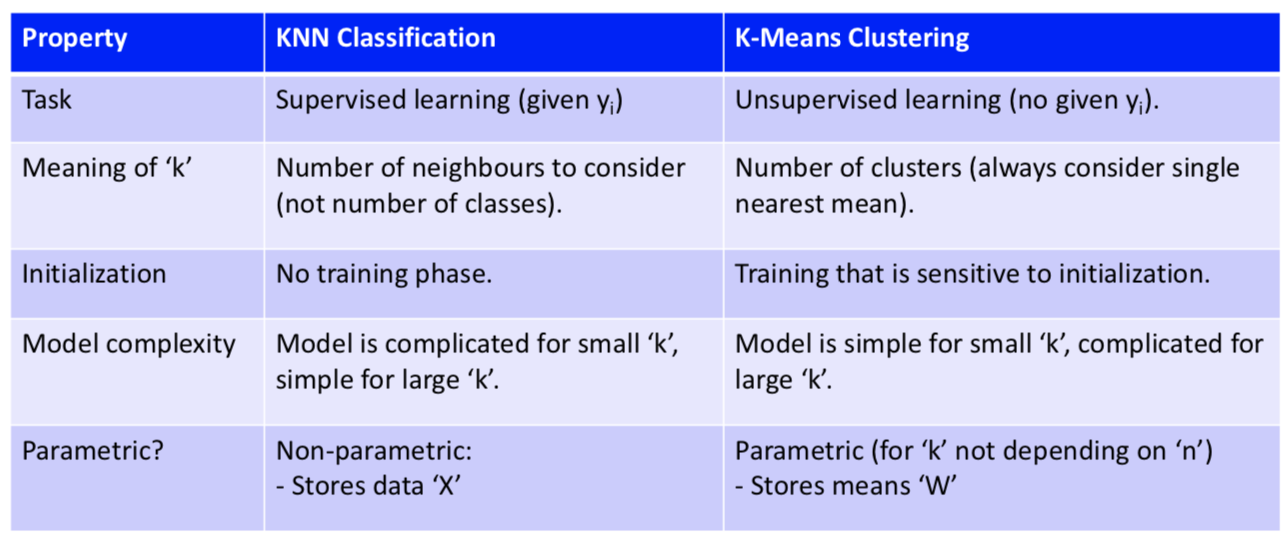
\includegraphics[width = 4.5in]{Pic9}
	\caption{Table showing the difference between KNN and K-means}
\end{figure}

\subsubsection*{What is $ K $-Means doing?}
We can interpret $ K $-means as minimizing an objective function, which is \gre{the sum of squared distances from each example $ x_i $ to its center $ w_{\hat{y_i}} $}:
\begin{align*}
\text{min.} \quad f(w_1, w_2, ..., w_k, \hat{y_1}, \hat{y_2}, ..., \hat{y_n}) &= \sum_{i = 1}^{n} \norm{w_{\hat{y_i}} - x_i}^2 
\end{align*}
In the above function, we have that $ w_{\hat{y_i}} $ is the cluster of example $ i $, therefore we have that $ \hat{y_i} \in \{1, ..., k\} $. Consequently the two $ k $-means steps are:
\begin{itemize}
	\item \gre{Minimize $ f $ in terms of the $ \hat{y_i} $} (i.e.: update the cluster assignments).
	\item \gre{Minimize $ f $ in terms of the $ w_c $} (i.e.: update the means)
\end{itemize}
\begin{figure}[H]
	\centering
	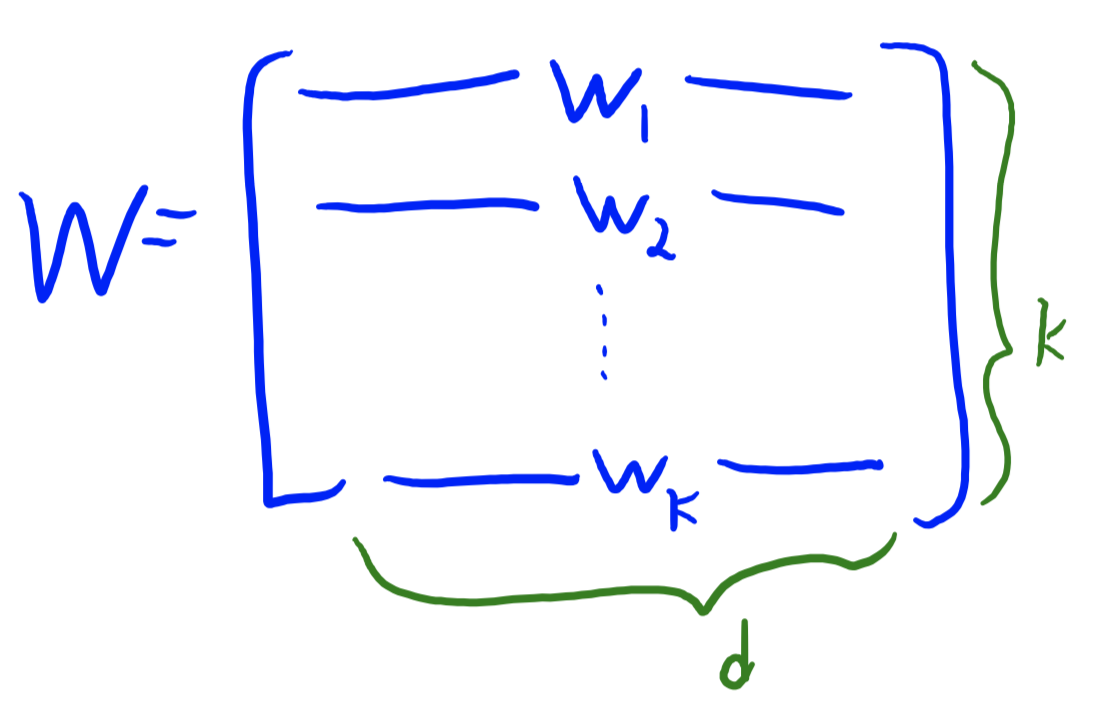
\includegraphics[width = 2in]{Pic10}
	\caption{Table showing the difference between KNN and K-means}
\end{figure}


The termination of the algorithm follows because:
\begin{itemize}
	\item Each step does not increase the objective.
	\item There are a finite number of assignments to k clusters.
\end{itemize}





\end{document}